\documentclass{beamer}
\usetheme{Darmstadt}

\setbeamertemplate{background canvas}[vertical shading][top=white, bottom=white!80!blue]
\setbeamertemplate{items}[circle]

\usepackage[utf8]{inputenc}
\usepackage[brazil]{babel}
\usepackage{hyperref}

\logo{
\includegraphics[scale=0.18]{images/pet_footer.png}}

\setbeamertemplate{sidebar left}{
  \logo{
\includegraphics[scale=0.08]{images/ufsc_footer.png}}
  \vfill
  \rlap{\hskip0.1cm\insertlogo}
  \vskip10pt
}

\title{UNIX e Linux}
\author{PET Computação}
\institute{Universidade Federal de Santa Catarina}
\date{\today}

\begin{document}
\maketitle

\section{Unix}
\subsection{Histórico}

\begin{frame}

  \begin{itemize}
  \item Criado no Bell Labs, em 1969.
  \item Seus criadores são Ken Thompson e Dennis Ritchie.
  \end{itemize}

  \begin{block}{Bell Labs}
    Laboratório onde foram criadas diversas coisas importantes para
    nós hoje:
    \begin{itemize}
    \item C/C++
    \item Transistor
    \item Laser
    \end{itemize}
  \end{block}

\end{frame}

\begin{frame}
  \begin{columns}
    \column{0.5\textwidth}

    \begin{block}{Dennis Ritchie}

      \begin{figure}
        \fbox{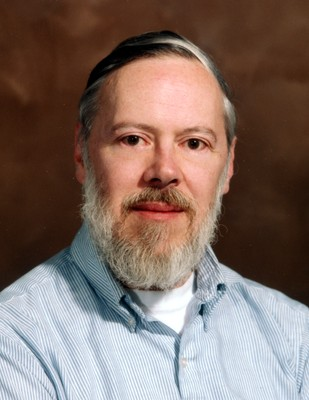
\includegraphics[scale=0.22]{images/dennis_ritchie.jpg}}
      \end{figure}

      \begin{itemize}
      \item B
      \item C
      \item MULTICS
      \end{itemize}

    \end{block}

    \column{0.5\textwidth}

    \begin{block}{Ken Thompson}

      \begin{figure}
        \fbox{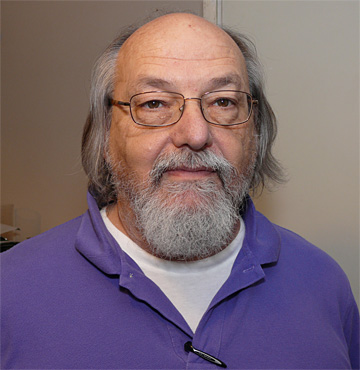
\includegraphics[scale=0.17]{images/ken_thompson.jpg}}
      \end{figure}

      \begin{itemize}
      \item B
      \item UTF-8
      \item Go
      \end{itemize}

    \end{block}
  \end{columns}
\end{frame}

\begin{frame}

  Hoje, ``Unix'' define uma família de sistemas operacionais que derivam
  do UNIX original.

  \begin{columns}

    \column{0.5\textwidth}
    
    \begin{block}{Unix}
      \begin{itemize}
      \item AIX
      \item Mac OS X
      \item HP-UX
      \item \ldots
      \end{itemize}
    \end{block}

    \column{0.5\textwidth}

    \begin{block}{Unix-like}
      \begin{itemize}
      \item FreeBSD
      \item GNU/Linux
      \item Minix
      \item \ldots
      \end{itemize}
    \end{block}

  \end{columns}

\end{frame}

\subsection{Usos atuais}

\begin{frame}
  
  Atualmente, sistemas Unix e Unix-like são utilizados em:

  \begin{itemize}
  \item Servidores
  \item Supercomputadores
  \item Computação pessoal
    \begin{itemize}
    \item Desktops
    \item Smartphones
    \end{itemize}
  \end{itemize}

\end{frame}

\section{GNU/Linux}

\begin{frame}
  Linux é um sistema Unix-like, de fácil acesso, e muito adequado à
  computação pessoal (e não só!)

  \begin{figure}
    
\includegraphics[scale=0.2]{images/tux.png}
    \footnotesize{
    \\Tux, mascote do Linux
    \\Créditos: Larry Ewing
    \\http://en.wikipedia.org/wiki/File:Tux-simple.svg
    }
  \end{figure}
\end{frame}

\subsection{Histórico}

\begin{frame}
  O kernel Linux foi criado por Linus Torvalds em 1991.

  \begin{columns}
    \column{0.25\textwidth}
    \column{0.5\textwidth}

    \begin{block}{Linus Torvalds}

      \begin{figure}
        \fbox{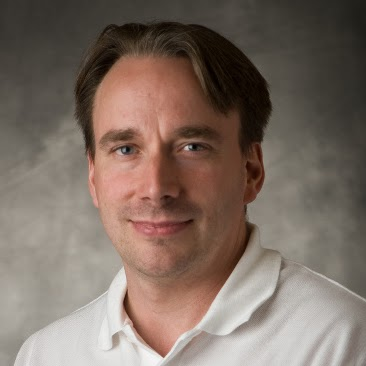
\includegraphics[scale=0.15]{images/linus_torvalds.jpg}}
      \end{figure}

      \begin{itemize}
      \item Kernel Linux
      \item Git
      \end{itemize}

    \end{block}

    \column{0.25\textwidth}
  \end{columns}

\end{frame}

\begin{frame}

  \begin{block}{Torvalds, comp.os.minix, 1991}
    \footnotesize{
      I'm doing a (free) operating system (just a hobby, won't be big and
      professional like gnu) for 386(486) AT clones.  This has been
      brewing since april, and is starting to get ready.  I'd like any
      feedback on things people like/dislike in minix, as my OS resembles
      it somewhat (same physical layout of the file-system (due to
      practical reasons) among other things).
      \newline
      \newline
      (\ldots)
      \newline
      \newline
      PS\@.  Yes - it's free of any minix code, and it has a
      multi-threaded fs. It is NOT protable (uses 386 task switching
      etc), and it probably never will support anything other than
      AT-harddisks, as that's all I have :-(. 
    }
  \end{block}

\end{frame}

\subsection{Kernel Linux e GNU}

\begin{frame}
  O projeto GNU, fundado por Richard Stallman, acabou adotando o kernel
  Linux como o kernel para seu sistema operacional, pois o HURD, o
  kernel que estava em desenvolvimento pela GNU estava em estágio muito
  inicial.
  
  \begin{columns}
    \column{0.25\textwidth}
    \column{0.5\textwidth}

    \begin{block}{Richard Matthew Stallman}

      \begin{figure}
        \fbox{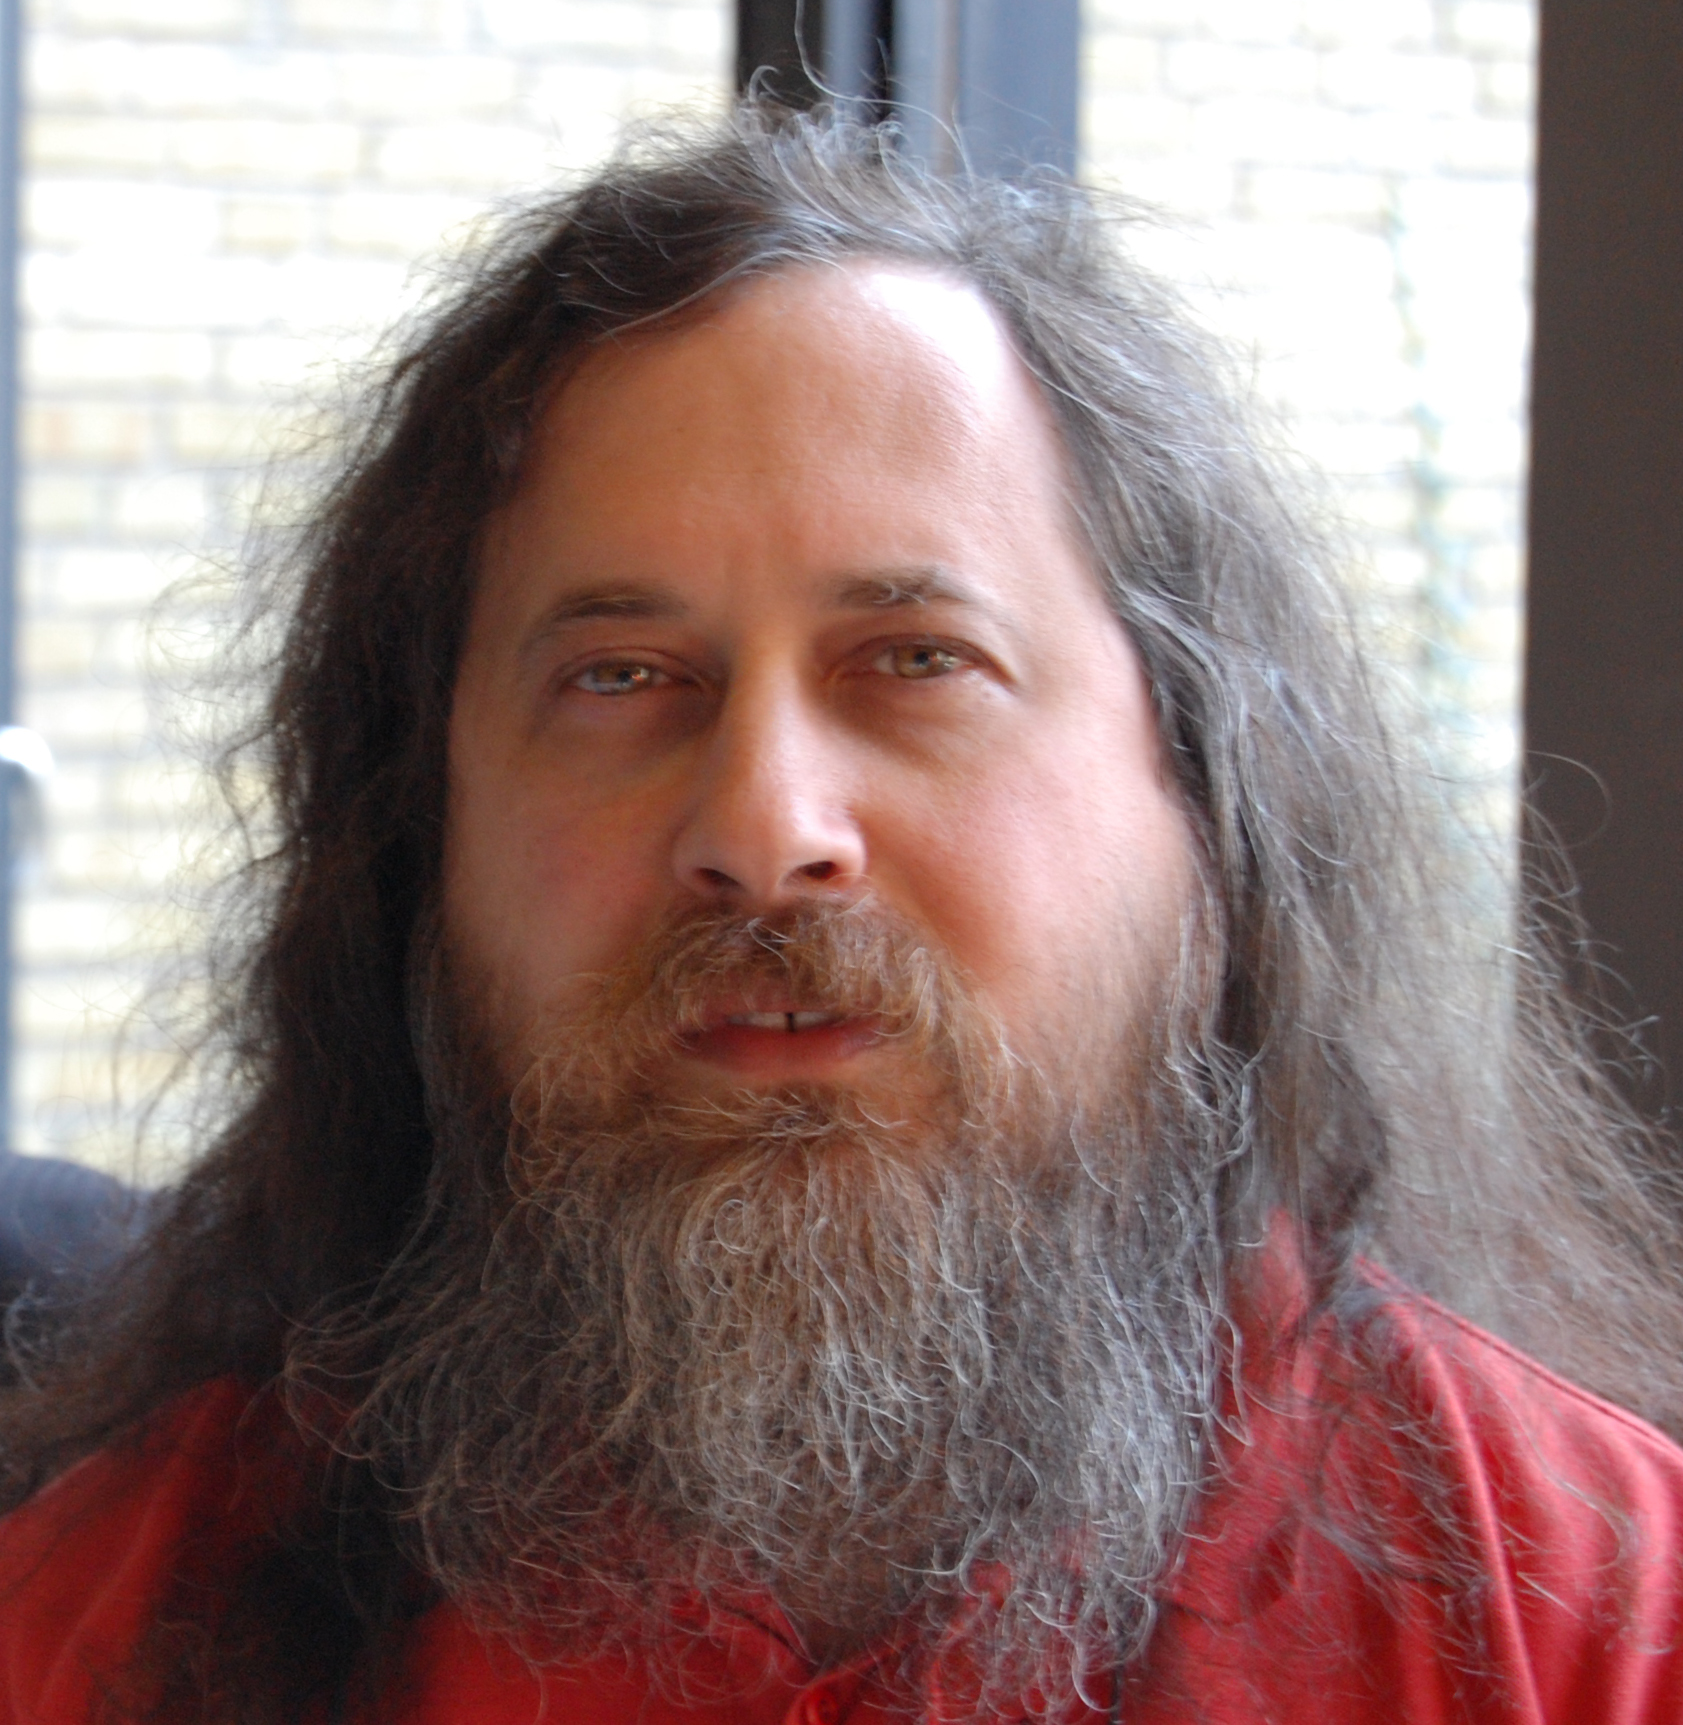
\includegraphics[scale=0.15]{images/richard_stallman.jpg}}
      \end{figure}

      \begin{itemize}
      \item GNU
      \item GNU Emacs
      \item POSIX
      \end{itemize}

    \end{block}

    \column{0.25\textwidth}
  \end{columns}
\end{frame}

\subsection{Distribuições}

\begin{frame}
  O sistema GNU/Linux possui várias distribuições. Uma distribuição
  nada mais é que um conjunto de softwares aplicativos em torno do
  kernel Linux e os utilitários GNU, de forma a atender um conjunto
  de usuários.

  \begin{columns}
    \column{0.2\textwidth}
    \column{0.6\textwidth}

    \begin{block}{Distribuições}
      \begin{itemize}
      \item Linux Mint
      \item Ubuntu
      \item Fedora
      \item Debian
      \item Arch Linux
      \item Slackware
      \item Gentoo
      \end{itemize}
    \end{block}

    \column{0.2\textwidth}
  \end{columns}

\end{frame}

\begin{frame}

  Toda distribuição é definida, basicamente, por como os programas
  disponíveis são empacotados e instalados. Na maior parte dos casos,
  isso é feito com um gerenciador de pacotes, como:

  \begin{itemize}
  \item portage
  \item pacman
  \item yum
  \item apt
  \end{itemize}

\end{frame}

\section{Hands-on}
\subsection{O terminal}

\frame{}

\section{}

\begin{frame}
  This work is licensed under the Creative Commons Attribution-ShareAlike 4.0 International License. To view a copy of this license, visit \url{http://creativecommons.org/licenses/by-sa/4.0/}.
\end{frame}

\end{document}
